
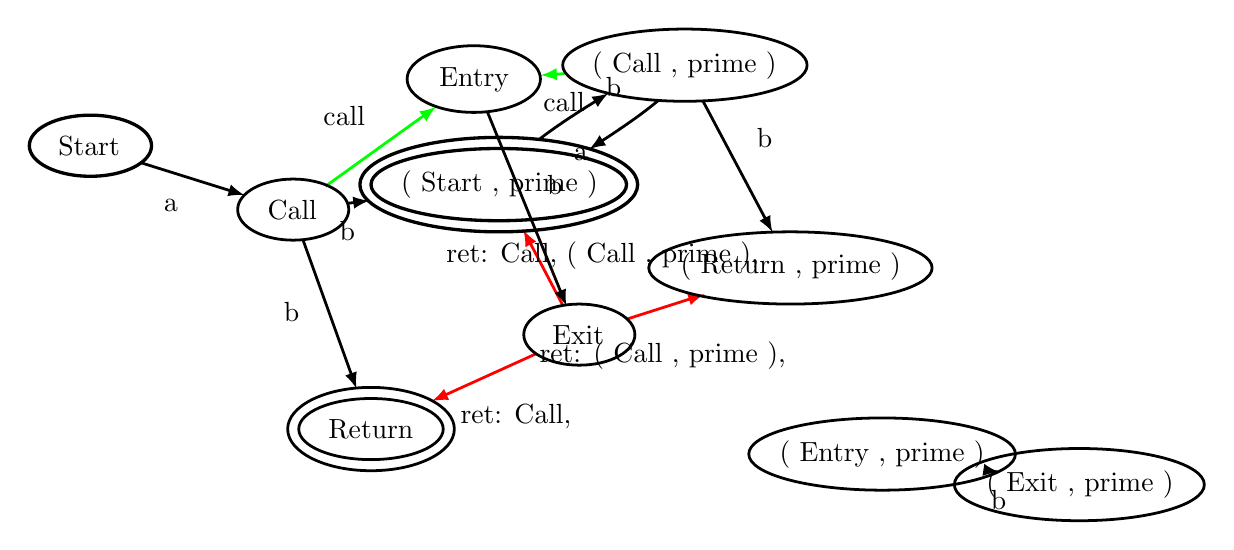
\begin{tikzpicture}[>=latex,line join=bevel,]
  \pgfsetlinewidth{1bp}
%%
\pgfsetcolor{black}
  % Edge: ( Call , prime ) -> Entry
  \pgfsetcolor{green}
  \draw [->] (194.67bp,162.94bp) .. controls (194.58bp,162.94bp) and (194.49bp,162.93bp)  .. (186.11bp,162.39bp);
  \definecolor{strokecol}{rgb}{0.0,0.0,0.0};
  \pgfsetstrokecolor{strokecol}
  \draw (194.53bp,152.93bp) node {call};
  % Edge: Exit -> Return
  \pgfsetcolor{red}
  \draw [->] (184.13bp,61.965bp) .. controls (176.06bp,58.304bp) and (165.88bp,53.689bp)  .. (146.91bp,45.084bp);
  \definecolor{strokecol}{rgb}{0.0,0.0,0.0};
  \pgfsetstrokecolor{strokecol}
  \draw (177.19bp,39.644bp) node {ret: Call, };
  % Edge: Call -> Entry
  \pgfsetcolor{green}
  \draw [->] (108.67bp,122.44bp) .. controls (117.44bp,128.74bp) and (129.58bp,137.46bp)  .. (148.39bp,150.98bp);
  \definecolor{strokecol}{rgb}{0.0,0.0,0.0};
  \pgfsetstrokecolor{strokecol}
  \draw (115.37bp,147.72bp) node {call};
  % Edge: ( Entry , prime ) -> ( Exit , prime )
  \draw [->] (350.83bp,19.514bp) .. controls (350.9bp,19.505bp) and (350.96bp,19.495bp)  .. (351.2bp,19.459bp);
  \draw (350.93bp,9.5bp) node {b};
  % Edge: Exit -> ( Return , prime )
  \pgfsetcolor{red}
  \draw [->] (216.96bp,74.531bp) .. controls (222.4bp,76.27bp) and (228.66bp,78.269bp)  .. (244.99bp,83.491bp);
  \definecolor{strokecol}{rgb}{0.0,0.0,0.0};
  \pgfsetstrokecolor{strokecol}
  \draw (229.99bp,61.416bp) node {ret: ( Call , prime ), };
  % Edge: Start -> Call
  \draw [->] (41.962bp,130.95bp) .. controls (50.418bp,128.3bp) and (60.601bp,125.11bp)  .. (79.463bp,119.2bp);
  \draw (52.92bp,115.58bp) node {a};
  % Edge: ( Call , prime ) -> ( Return , prime )
  \draw [->] (244.49bp,153.12bp) .. controls (250.09bp,142.55bp) and (258.22bp,127.22bp)  .. (269.53bp,105.89bp);
  \draw (266.66bp,139.93bp) node {b};
  % Edge: Exit -> ( Start , prime )
  \pgfsetcolor{red}
  \draw [->] (194.14bp,79.39bp) .. controls (191.41bp,84.579bp) and (187.99bp,91.102bp)  .. (179.84bp,106.65bp);
  \definecolor{strokecol}{rgb}{0.0,0.0,0.0};
  \pgfsetstrokecolor{strokecol}
  \draw (208.38bp,97.45bp) node {ret: Call, ( Call , prime ), };
  % Edge: Entry -> Exit
  \draw [->] (166.88bp,149.22bp) .. controls (173.07bp,134.05bp) and (183.98bp,107.3bp)  .. (195.35bp,79.389bp);
  \draw (191.18bp,123.05bp) node {b};
  % Edge: Call -> ( Start , prime )
  \draw [->] (116.27bp,116.22bp) .. controls (116.43bp,116.24bp) and (116.59bp,116.26bp)  .. (124.41bp,117.22bp);
  \draw (116.51bp,106.25bp) node {b};
  % Edge: Call -> Return
  \draw [->] (100.48bp,103.2bp) .. controls (104.52bp,91.953bp) and (111.04bp,73.817bp)  .. (119.76bp,49.568bp);
  \draw (96.407bp,77.146bp) node {b};
  % Edge: ( Call , prime ) -> ( Start , prime )
  \draw [->] (228.51bp,153.35bp) .. controls (223.97bp,149.53bp) and (218.2bp,145.29bp)  .. (203.59bp,135.77bp);
  \draw (212.29bp,158.28bp) node {b};
  % Edge: ( Start , prime ) -> ( Call , prime )
  \draw [->] (185.17bp,139.02bp) .. controls (190.11bp,142.82bp) and (195.9bp,146.84bp)  .. (210.45bp,155.86bp);
  \draw (200.49bp,133.81bp) node {a};
  % Node: Return
\begin{scope}
  \definecolor{strokecol}{rgb}{0.0,0.0,0.0};
  \pgfsetstrokecolor{strokecol}
  \draw (125bp,35bp) ellipse (26bp and 11bp);
  \draw (125bp,35bp) ellipse (30bp and 15bp);
  \draw (124.95bp,35.125bp) node {Return};
\end{scope}
  % Node: ( Start , prime )
\begin{scope}
  \definecolor{strokecol}{rgb}{0.0,0.0,0.0};
  \pgfsetstrokecolor{strokecol}
  \draw [very thick] (171bp,123bp) ellipse (46bp and 13bp);
  \draw [very thick] (171bp,123bp) ellipse (50bp and 17bp);
  \draw (171.27bp,122.97bp) node {( Start , prime )};
\end{scope}
  % Node: Exit
\begin{scope}
  \definecolor{strokecol}{rgb}{0.0,0.0,0.0};
  \pgfsetstrokecolor{strokecol}
  \draw (200bp,69bp) ellipse (20bp and 11bp);
  \draw (199.6bp,68.98bp) node {Exit};
\end{scope}
  % Node: ( Call , prime )
\begin{scope}
  \definecolor{strokecol}{rgb}{0.0,0.0,0.0};
  \pgfsetstrokecolor{strokecol}
  \draw (238bp,166bp) ellipse (44bp and 13bp);
  \draw (237.81bp,165.71bp) node {( Call , prime )};
\end{scope}
  % Node: ( Exit , prime )
\begin{scope}
  \definecolor{strokecol}{rgb}{0.0,0.0,0.0};
  \pgfsetstrokecolor{strokecol}
  \draw (380bp,15bp) ellipse (45bp and 13bp);
  \draw (380.21bp,15.125bp) node {( Exit , prime )};
\end{scope}
  % Node: ( Entry , prime )
\begin{scope}
  \definecolor{strokecol}{rgb}{0.0,0.0,0.0};
  \pgfsetstrokecolor{strokecol}
  \draw (309bp,26bp) ellipse (48bp and 13bp);
  \draw (309bp,25.764bp) node {( Entry , prime )};
\end{scope}
  % Node: Start
\begin{scope}
  \definecolor{strokecol}{rgb}{0.0,0.0,0.0};
  \pgfsetstrokecolor{strokecol}
  \draw [very thick] (24bp,137bp) ellipse (22bp and 11bp);
  \draw (23.5bp,136.73bp) node {Start};
\end{scope}
  % Node: Call
\begin{scope}
  \definecolor{strokecol}{rgb}{0.0,0.0,0.0};
  \pgfsetstrokecolor{strokecol}
  \draw (97bp,114bp) ellipse (20bp and 11bp);
  \draw (96.662bp,113.81bp) node {Call};
\end{scope}
  % Node: Entry
\begin{scope}
  \definecolor{strokecol}{rgb}{0.0,0.0,0.0};
  \pgfsetstrokecolor{strokecol}
  \draw (162bp,161bp) ellipse (24bp and 12bp);
  \draw (162.14bp,160.86bp) node {Entry};
\end{scope}
  % Node: ( Return , prime )
\begin{scope}
  \definecolor{strokecol}{rgb}{0.0,0.0,0.0};
  \pgfsetstrokecolor{strokecol}
  \draw (276bp,93bp) ellipse (51bp and 13bp);
  \draw (276.12bp,93.442bp) node {( Return , prime )};
\end{scope}
%
\end{tikzpicture}
